\documentclass[main.tex]{subfile}

\begin{document}

\section{Model Predictive Controllers} 
\label{sec:sbmpc}

SBMPC is an extension of the MPC algorithm and therefore we first review the
basics MPC so as to aid in understanding SBMPC. A basic MPC algorithm is as
follows\cite{autoVehicle}:

\begin{enumerate}
	\item Obtain the current state of the system being controlled.
	\item Determine the optimal control inputs ($u_{t+1,t+2,...,t+N}$) by solving
		an optimization problem that compares the predicted system output with a
		desired system output while satisfying system constraints.
	\item Send the first generated control input $u_{t+1}$ to the plant, update
		the system state variable and then repeat the process until the system has
		reached the desired goal or state (depending on the application).
\end{enumerate}

This algorithm can be explained through an example. Suppose that we wish to fire
a rifle at a moving target. We could generate a kinematic model for our system
and generate some constraints (such as the bullet must be restricted to a
certain trajectory to avoid damaging property or humans). Our system inputs
would be the angle of the rifle both vertically and horizontally. The state
could be the kinetic and kinematic properties of the bullet and target. The
system output would be the location of the bullet relative to the target.
\figref{example} shows this situation. At some time $t=0$ the target is moving.
The SBMPC control system then predicts where the target would be at time
$t=t_{\texttt{hit}}$ and then attempts a shot. 

\begin{figure}[H]
	\begin{center}
		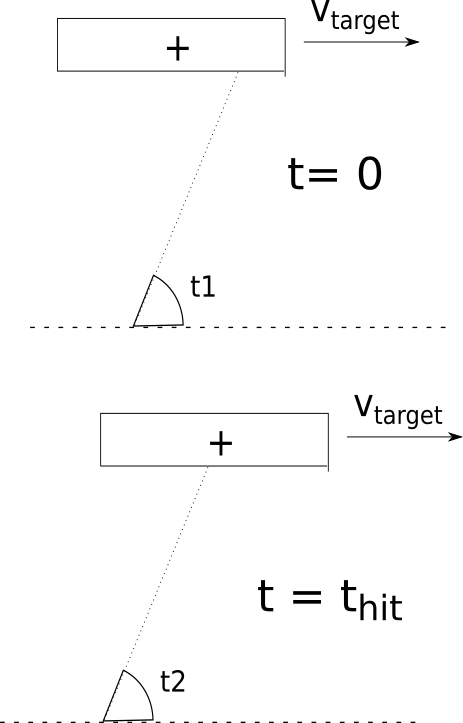
\includegraphics[width=\linewidth]{example.png}
	\end{center}
	\caption{Target Tracking Gun example with SBMPC}
	\label{fig:example}
\end{figure}

For the sake of the example let us assume that we can freeze the system at
anytime wherein our clock will also stop. To get hit on the target we first,
freeze our system. Then we calculate an optimal set of system inputs for the
next $N$ time steps while obeying our system constraints. Once an optimal
predicted trajectory is determined we then implement our first set of these
system inputs while unfreezing our system. Practically, in industry, the system
is actually never "frozen" but the prediction step is performed fast enough that
the system is assumed to not have changed in its state while computing the
prediction.

% section sbmpc (end)

\section{Sample Based Model Predictive Controllers} 
\label{sec:sample_based_model_predictive_controllers}

We now explain the "sample-based" part of SBMPC. It was discovered that
sampling-based motion planning algorithms are great for solving basic
optimization problems. Such algorithms include rapidly exploring random trees,
and \Astar algorithms. Both algorithms were designed for sampling some
search-space and generating a graph that contained an optimal path for some
start and goal nodes. For MPC we use these methods for the optimization step
which yield faster path planning times, and more reliable path planning results.

The novel algorithm is based on the \Astar algorithm where the nodes are control
state configurations and edges are the system inputs to transform the system
from one control state to the next.  This sampling optimization algorithm as
discussed in \cite{uphill} is as follows: 

\begin{enumerate}
	\item Generate a set of samples of the control space.
	\item Use the generated control space samples to generate state-space samples.
	\item Use an \Astar like heuristic to evaluate the cost of each node based on
		the desired objective.
	\item Iterate through the nodes (starting with the lowest cost node first) and
		compute the edge cost for that node starting from the current node. Stop
		when an edge cost is evaluated that fits the system constraints.
	\item Continue the process until the system has reached its goal.
\end{enumerate}

% section sample_based_model_predictive_controllers (end)

\end{document}
